\documentclass[twoside]{book}

% Packages required by doxygen
\usepackage{fixltx2e}
\usepackage{calc}
\usepackage{doxygen}
\usepackage[export]{adjustbox} % also loads graphicx
\usepackage{graphicx}
\usepackage[utf8]{inputenc}
\usepackage{makeidx}
\usepackage{multicol}
\usepackage{multirow}
\PassOptionsToPackage{warn}{textcomp}
\usepackage{textcomp}
\usepackage[nointegrals]{wasysym}
\usepackage[table]{xcolor}

% Font selection
\usepackage[T1]{fontenc}
\usepackage[scaled=.90]{helvet}
\usepackage{courier}
\usepackage{amssymb}
\usepackage{sectsty}
\renewcommand{\familydefault}{\sfdefault}
\allsectionsfont{%
  \fontseries{bc}\selectfont%
  \color{darkgray}%
}
\renewcommand{\DoxyLabelFont}{%
  \fontseries{bc}\selectfont%
  \color{darkgray}%
}
\newcommand{\+}{\discretionary{\mbox{\scriptsize$\hookleftarrow$}}{}{}}

% Page & text layout
\usepackage{geometry}
\geometry{%
  a4paper,%
  top=2.5cm,%
  bottom=2.5cm,%
  left=2.5cm,%
  right=2.5cm%
}
\tolerance=750
\hfuzz=15pt
\hbadness=750
\setlength{\emergencystretch}{15pt}
\setlength{\parindent}{0cm}
\setlength{\parskip}{3ex plus 2ex minus 2ex}
\makeatletter
\renewcommand{\paragraph}{%
  \@startsection{paragraph}{4}{0ex}{-1.0ex}{1.0ex}{%
    \normalfont\normalsize\bfseries\SS@parafont%
  }%
}
\renewcommand{\subparagraph}{%
  \@startsection{subparagraph}{5}{0ex}{-1.0ex}{1.0ex}{%
    \normalfont\normalsize\bfseries\SS@subparafont%
  }%
}
\makeatother

% Headers & footers
\usepackage{fancyhdr}
\pagestyle{fancyplain}
\fancyhead[LE]{\fancyplain{}{\bfseries\thepage}}
\fancyhead[CE]{\fancyplain{}{}}
\fancyhead[RE]{\fancyplain{}{\bfseries\leftmark}}
\fancyhead[LO]{\fancyplain{}{\bfseries\rightmark}}
\fancyhead[CO]{\fancyplain{}{}}
\fancyhead[RO]{\fancyplain{}{\bfseries\thepage}}
\fancyfoot[LE]{\fancyplain{}{}}
\fancyfoot[CE]{\fancyplain{}{}}
\fancyfoot[RE]{\fancyplain{}{\bfseries\scriptsize Generated by Doxygen }}
\fancyfoot[LO]{\fancyplain{}{\bfseries\scriptsize Generated by Doxygen }}
\fancyfoot[CO]{\fancyplain{}{}}
\fancyfoot[RO]{\fancyplain{}{}}
\renewcommand{\footrulewidth}{0.4pt}
\renewcommand{\chaptermark}[1]{%
  \markboth{#1}{}%
}
\renewcommand{\sectionmark}[1]{%
  \markright{\thesection\ #1}%
}

% Indices & bibliography
\usepackage{natbib}
\usepackage[titles]{tocloft}
\setcounter{tocdepth}{3}
\setcounter{secnumdepth}{5}
\makeindex

% Hyperlinks (required, but should be loaded last)
\usepackage{ifpdf}
\ifpdf
  \usepackage[pdftex,pagebackref=true]{hyperref}
\else
  \usepackage[ps2pdf,pagebackref=true]{hyperref}
\fi
\hypersetup{%
  colorlinks=true,%
  linkcolor=blue,%
  citecolor=blue,%
  unicode%
}

% Custom commands
\newcommand{\clearemptydoublepage}{%
  \newpage{\pagestyle{empty}\cleardoublepage}%
}

\usepackage{caption}
\captionsetup{labelsep=space,justification=centering,font={bf},singlelinecheck=off,skip=4pt,position=top}

%===== C O N T E N T S =====

\begin{document}

% Titlepage & ToC
\hypersetup{pageanchor=false,
             bookmarksnumbered=true,
             pdfencoding=unicode
            }
\pagenumbering{alph}
\begin{titlepage}
\vspace*{7cm}
\begin{center}%
{\Large time\+\_\+series }\\
\vspace*{1cm}
{\large Generated by Doxygen 1.8.13}\\
\end{center}
\end{titlepage}
\clearemptydoublepage
\pagenumbering{roman}
\tableofcontents
\clearemptydoublepage
\pagenumbering{arabic}
\hypersetup{pageanchor=true}

%--- Begin generated contents ---
\chapter{Time Series}
\label{md_readme}
\Hypertarget{md_readme}
\subsection*{What is it}

Dynamic graph \char`\"{}glue code\char`\"{} responsible for the instanciation of the graph and the python interpreter. Provide a R\+OS server in order to create distant R\+OS clients.

\subsection*{Authors}


\begin{DoxyItemize}
\item Maximilien Naveau
\item Julian Viereck
\item Andrea Delprete
\end{DoxyItemize}

\subsection*{Copyrights}

Copyright (c) 2019, New York University and Max Planck Gesellschaft.

\subsection*{License}

License B\+S\+D-\/3-\/\+Clause

\subsection*{Installation\+:}

This is a ros package so it should be in a R\+OS environment. One can still test its compilation by using the following instruction\+:

`cd \hyperlink{namespacedynamic__graph__manager}{dynamic\+\_\+graph\+\_\+manager} mkdir \+\_\+build cd \+\_\+build cmake .. make -\/j8`

\subsection*{Usage\+:}

Inherite from the class Dynamic\+Graph\+Manager and overload the three functions responsible for the hardware\+: \begin{DoxyVerb} `virtual void initialize_hardware_communication_process()`

 `virtual void get_sensors_to_map(VectorDGMap&)`
\end{DoxyVerb}


and \begin{DoxyVerb}`virtual void set_motor_controls_from_map(const VectorDGMap&)`
\end{DoxyVerb}


\subsection*{Documentation\+:}

See demo and unit tests for more information on the A\+PI. Doxygen informations are available by calling\+: \begin{DoxyVerb}`catkin_make -DBUILD_DOCUMENTATION=ON`\end{DoxyVerb}
 
\chapter{Hierarchical Index}
\section{Class Hierarchy}
This inheritance list is sorted roughly, but not completely, alphabetically\+:\begin{DoxyCompactList}
\item array\+\_\+members\begin{DoxyCompactList}
\item \contentsline{section}{shared\+\_\+memory\+:\+:array$<$ T, S\+I\+ZE $>$}{\pageref{classshared__memory_1_1array}}{}
\end{DoxyCompactList}
\item \contentsline{section}{shared\+\_\+memory\+:\+:Condition\+Variable}{\pageref{classshared__memory_1_1ConditionVariable}}{}
\item \contentsline{section}{Config}{\pageref{classConfig}}{}
\item exception\begin{DoxyCompactList}
\item \contentsline{section}{shared\+\_\+memory\+:\+:Allocation\+\_\+exception}{\pageref{classshared__memory_1_1Allocation__exception}}{}
\item \contentsline{section}{shared\+\_\+memory\+:\+:Memory\+\_\+overflow\+\_\+exception}{\pageref{classshared__memory_1_1Memory__overflow__exception}}{}
\item \contentsline{section}{shared\+\_\+memory\+:\+:Not\+\_\+consumed\+\_\+exception}{\pageref{classshared__memory_1_1Not__consumed__exception}}{}
\item \contentsline{section}{shared\+\_\+memory\+:\+:Unexpected\+\_\+map\+\_\+key$<$ Key $>$}{\pageref{classshared__memory_1_1Unexpected__map__key}}{}
\item \contentsline{section}{shared\+\_\+memory\+:\+:Unexpected\+\_\+size\+\_\+exception}{\pageref{classshared__memory_1_1Unexpected__size__exception}}{}
\end{DoxyCompactList}
\item \contentsline{section}{shared\+\_\+memory\+:\+:Exchange\+\_\+manager\+\_\+consumer$<$ Serializable, Q\+U\+E\+U\+E\+\_\+\+S\+I\+ZE $>$}{\pageref{classshared__memory_1_1Exchange__manager__consumer}}{}
\item \contentsline{section}{shared\+\_\+memory\+:\+:Exchange\+\_\+manager\+\_\+producer$<$ Serializable, Q\+U\+E\+U\+E\+\_\+\+S\+I\+ZE $>$}{\pageref{classshared__memory_1_1Exchange__manager__producer}}{}
\item \contentsline{section}{shared\+\_\+memory\+:\+:Four\+\_\+int\+\_\+values}{\pageref{classshared__memory_1_1Four__int__values}}{}
\item \contentsline{section}{shared\+\_\+memory\+:\+:Item$<$ S\+I\+ZE $>$}{\pageref{classshared__memory_1_1Item}}{}
\item \contentsline{section}{shared\+\_\+memory\+:\+:Lock}{\pageref{classshared__memory_1_1Lock}}{}
\item \contentsline{section}{shared\+\_\+memory\+:\+:Locked\+Condition\+Variable}{\pageref{classshared__memory_1_1LockedConditionVariable}}{}
\item \contentsline{section}{Measure\+Time}{\pageref{structMeasureTime}}{}
\item \contentsline{section}{shared\+\_\+memory\+:\+:Mutex}{\pageref{classshared__memory_1_1Mutex}}{}
\item \contentsline{section}{shared\+\_\+memory\+:\+:Segment\+Info}{\pageref{classshared__memory_1_1SegmentInfo}}{}
\item \contentsline{section}{Serializable$<$ S\+I\+ZE $>$}{\pageref{classSerializable}}{}
\item \contentsline{section}{shared\+\_\+memory\+:\+:Serializable\+\_\+exchange$<$ Serializable $>$}{\pageref{classshared__memory_1_1Serializable__exchange}}{}
\item \contentsline{section}{Serializable\+Example}{\pageref{classSerializableExample}}{}
\item \contentsline{section}{shared\+\_\+memory\+:\+:Serializer$<$ Serializable $>$}{\pageref{classshared__memory_1_1Serializer}}{}
\item \contentsline{section}{shared\+\_\+memory\+:\+:Shared\+Memory\+Segment}{\pageref{classshared__memory_1_1SharedMemorySegment}}{}
\item \contentsline{section}{shared\+\_\+memory\+:\+:Shm\+Type\+Helper$<$ Elem\+Type $>$}{\pageref{structshared__memory_1_1ShmTypeHelper}}{}
\end{DoxyCompactList}

\chapter{Class Index}
\section{Class List}
Here are the classes, structs, unions and interfaces with brief descriptions\+:\begin{DoxyCompactList}
\item\contentsline{section}{\hyperlink{classshared__memory_1_1Allocation__exception}{shared\+\_\+memory\+::\+Allocation\+\_\+exception} }{\pageref{classshared__memory_1_1Allocation__exception}}{}
\item\contentsline{section}{\hyperlink{classshared__memory_1_1array}{shared\+\_\+memory\+::array$<$ T, S\+I\+Z\+E $>$} \\*Implement a shared array stored on a shared memory segment }{\pageref{classshared__memory_1_1array}}{}
\item\contentsline{section}{\hyperlink{classshared__memory_1_1internal_1_1array__members}{shared\+\_\+memory\+::internal\+::array\+\_\+members$<$ T, S\+I\+Z\+E, Enable $>$} }{\pageref{classshared__memory_1_1internal_1_1array__members}}{}
\item\contentsline{section}{\hyperlink{classshared__memory_1_1internal_1_1array__members_3_01T_00_010_00_01typename_01std_1_1enable__ifb2fde5f96702510d664610c5e9570772}{shared\+\_\+memory\+::internal\+::array\+\_\+members$<$ T, 0, typename std\+::enable\+\_\+if$<$ std\+::is\+\_\+fundamental$<$ T $>$\+::value $>$\+::type $>$} }{\pageref{classshared__memory_1_1internal_1_1array__members_3_01T_00_010_00_01typename_01std_1_1enable__ifb2fde5f96702510d664610c5e9570772}}{}
\item\contentsline{section}{\hyperlink{classshared__memory_1_1internal_1_1array__members_3_01T_00_01SIZE_00_01typename_01std_1_1enable_de9984c52d14535c26d7a424fbd87fe2}{shared\+\_\+memory\+::internal\+::array\+\_\+members$<$ T, S\+I\+Z\+E, typename std\+::enable\+\_\+if$<$ std\+::is\+\_\+fundamental$<$ T $>$\+::value \&\&\+S\+I\+Z\+E!=0 $>$\+::type $>$} }{\pageref{classshared__memory_1_1internal_1_1array__members_3_01T_00_01SIZE_00_01typename_01std_1_1enable_de9984c52d14535c26d7a424fbd87fe2}}{}
\item\contentsline{section}{\hyperlink{classshared__memory_1_1ConditionVariable}{shared\+\_\+memory\+::\+Condition\+Variable} }{\pageref{classshared__memory_1_1ConditionVariable}}{}
\item\contentsline{section}{\hyperlink{classConfig}{Config} }{\pageref{classConfig}}{}
\item\contentsline{section}{\hyperlink{classshared__memory_1_1Exchange__manager__consumer}{shared\+\_\+memory\+::\+Exchange\+\_\+manager\+\_\+consumer$<$ Serializable, Q\+U\+E\+U\+E\+\_\+\+S\+I\+Z\+E $>$} }{\pageref{classshared__memory_1_1Exchange__manager__consumer}}{}
\item\contentsline{section}{\hyperlink{classshared__memory_1_1internal_1_1Exchange__manager__memory}{shared\+\_\+memory\+::internal\+::\+Exchange\+\_\+manager\+\_\+memory$<$ Serializable, Q\+U\+E\+U\+E\+\_\+\+S\+I\+Z\+E $>$} }{\pageref{classshared__memory_1_1internal_1_1Exchange__manager__memory}}{}
\item\contentsline{section}{\hyperlink{classshared__memory_1_1Exchange__manager__producer}{shared\+\_\+memory\+::\+Exchange\+\_\+manager\+\_\+producer$<$ Serializable, Q\+U\+E\+U\+E\+\_\+\+S\+I\+Z\+E $>$} }{\pageref{classshared__memory_1_1Exchange__manager__producer}}{}
\item\contentsline{section}{\hyperlink{classshared__memory_1_1Four__int__values}{shared\+\_\+memory\+::\+Four\+\_\+int\+\_\+values} \\*Example of an instance that can be serialized }{\pageref{classshared__memory_1_1Four__int__values}}{}
\item\contentsline{section}{\hyperlink{classshared__memory_1_1Item}{shared\+\_\+memory\+::\+Item$<$ S\+I\+Z\+E $>$} }{\pageref{classshared__memory_1_1Item}}{}
\item\contentsline{section}{\hyperlink{classshared__memory_1_1Lock}{shared\+\_\+memory\+::\+Lock} \\*A scope lock object for locking a shared memory mutex, to use for example with a shared memory condition variable }{\pageref{classshared__memory_1_1Lock}}{}
\item\contentsline{section}{\hyperlink{classshared__memory_1_1LockedConditionVariable}{shared\+\_\+memory\+::\+Locked\+Condition\+Variable} \\*Here as a anonymous layer on top of the boost intersprocess condition variable labrary }{\pageref{classshared__memory_1_1LockedConditionVariable}}{}
\item\contentsline{section}{\hyperlink{structMeasureTime}{Measure\+Time} }{\pageref{structMeasureTime}}{}
\item\contentsline{section}{\hyperlink{classshared__memory_1_1Memory__overflow__exception}{shared\+\_\+memory\+::\+Memory\+\_\+overflow\+\_\+exception} }{\pageref{classshared__memory_1_1Memory__overflow__exception}}{}
\item\contentsline{section}{\hyperlink{classshared__memory_1_1Mutex}{shared\+\_\+memory\+::\+Mutex} }{\pageref{classshared__memory_1_1Mutex}}{}
\item\contentsline{section}{\hyperlink{classshared__memory_1_1Not__consumed__exception}{shared\+\_\+memory\+::\+Not\+\_\+consumed\+\_\+exception} }{\pageref{classshared__memory_1_1Not__consumed__exception}}{}
\item\contentsline{section}{\hyperlink{classshared__memory_1_1SegmentInfo}{shared\+\_\+memory\+::\+Segment\+Info} \\*Encapsulate information related to a shared memory segment }{\pageref{classshared__memory_1_1SegmentInfo}}{}
\item\contentsline{section}{\hyperlink{classSerializable}{Serializable$<$ S\+I\+Z\+E $>$} }{\pageref{classSerializable}}{}
\item\contentsline{section}{\hyperlink{classshared__memory_1_1Serializable__exchange}{shared\+\_\+memory\+::\+Serializable\+\_\+exchange$<$ Serializable $>$} }{\pageref{classshared__memory_1_1Serializable__exchange}}{}
\item\contentsline{section}{\hyperlink{classSerializableExample}{Serializable\+Example} }{\pageref{classSerializableExample}}{}
\item\contentsline{section}{\hyperlink{classshared__memory_1_1internal_1_1Serialized__read}{shared\+\_\+memory\+::internal\+::\+Serialized\+\_\+read$<$ Serializable $>$} }{\pageref{classshared__memory_1_1internal_1_1Serialized__read}}{}
\item\contentsline{section}{\hyperlink{classshared__memory_1_1internal_1_1Serialized__write}{shared\+\_\+memory\+::internal\+::\+Serialized\+\_\+write$<$ Serializable $>$} }{\pageref{classshared__memory_1_1internal_1_1Serialized__write}}{}
\item\contentsline{section}{\hyperlink{classshared__memory_1_1Serializer}{shared\+\_\+memory\+::\+Serializer$<$ Serializable $>$} }{\pageref{classshared__memory_1_1Serializer}}{}
\item\contentsline{section}{\hyperlink{classshared__memory_1_1SharedMemorySegment}{shared\+\_\+memory\+::\+Shared\+Memory\+Segment} \\*The \hyperlink{classshared__memory_1_1SharedMemorySegment}{Shared\+Memory\+Segment} contains the pointers of the shared objects in on shared memrory segment }{\pageref{classshared__memory_1_1SharedMemorySegment}}{}
\item\contentsline{section}{\hyperlink{structshared__memory_1_1ShmTypeHelper}{shared\+\_\+memory\+::\+Shm\+Type\+Helper$<$ Elem\+Type $>$} \\*\hyperlink{structshared__memory_1_1ShmTypeHelper}{Shm\+Type\+Helper} is a small struct that allow the definition of templated typedef }{\pageref{structshared__memory_1_1ShmTypeHelper}}{}
\item\contentsline{section}{\hyperlink{classshared__memory_1_1Unexpected__map__key}{shared\+\_\+memory\+::\+Unexpected\+\_\+map\+\_\+key$<$ Key $>$} }{\pageref{classshared__memory_1_1Unexpected__map__key}}{}
\item\contentsline{section}{\hyperlink{classshared__memory_1_1Unexpected__size__exception}{shared\+\_\+memory\+::\+Unexpected\+\_\+size\+\_\+exception} }{\pageref{classshared__memory_1_1Unexpected__size__exception}}{}
\end{DoxyCompactList}

\chapter{File Index}
\section{File List}
Here is a list of all documented files with brief descriptions\+:\begin{DoxyCompactList}
\item\contentsline{section}{include/dg\+\_\+blmc\+\_\+robots/\hyperlink{common__header_8hpp}{common\+\_\+header.\+hpp} }{\pageref{common__header_8hpp}}{}
\item\contentsline{section}{include/dg\+\_\+blmc\+\_\+robots/\hyperlink{dgm__single__motor_8hpp}{dgm\+\_\+single\+\_\+motor.\+hpp} }{\pageref{dgm__single__motor_8hpp}}{}
\item\contentsline{section}{include/dg\+\_\+blmc\+\_\+robots/{\bfseries dgm\+\_\+solo12.\+hpp} }{\pageref{dgm__solo12_8hpp}}{}
\item\contentsline{section}{include/dg\+\_\+blmc\+\_\+robots/{\bfseries dgm\+\_\+solo8.\+hpp} }{\pageref{dgm__solo8_8hpp}}{}
\item\contentsline{section}{include/dg\+\_\+blmc\+\_\+robots/{\bfseries dgm\+\_\+solo8ti.\+hpp} }{\pageref{dgm__solo8ti_8hpp}}{}
\item\contentsline{section}{include/dg\+\_\+blmc\+\_\+robots/{\bfseries dgm\+\_\+solo\+\_\+simple\+\_\+simu.\+hpp} }{\pageref{dgm__solo__simple__simu_8hpp}}{}
\item\contentsline{section}{include/dg\+\_\+blmc\+\_\+robots/\hyperlink{dgm__stuggihop_8hpp}{dgm\+\_\+stuggihop.\+hpp} }{\pageref{dgm__stuggihop_8hpp}}{}
\item\contentsline{section}{include/dg\+\_\+blmc\+\_\+robots/{\bfseries dgm\+\_\+teststand.\+hpp} }{\pageref{dgm__teststand_8hpp}}{}
\item\contentsline{section}{src/\hyperlink{dgm__solo__simple__simu_8cpp}{dgm\+\_\+solo\+\_\+simple\+\_\+simu.\+cpp} \\*The hardware wrapper of the solo naive simulation }{\pageref{dgm__solo__simple__simu_8cpp}}{}
\item\contentsline{section}{src/\hyperlink{dgm__stuggihop_8cpp}{dgm\+\_\+stuggihop.\+cpp} \\*D\+GM wrapper around the stuggihop robot }{\pageref{dgm__stuggihop_8cpp}}{}
\end{DoxyCompactList}

\chapter{Class Documentation}
\hypertarget{classtime__series_1_1MultiprocessTimeSeries}{}\section{time\+\_\+series\+:\+:Multiprocess\+Time\+Series$<$ T $>$ Class Template Reference}
\label{classtime__series_1_1MultiprocessTimeSeries}\index{time\+\_\+series\+::\+Multiprocess\+Time\+Series$<$ T $>$@{time\+\_\+series\+::\+Multiprocess\+Time\+Series$<$ T $>$}}


Multiprocess Time Series.  




{\ttfamily \#include $<$multiprocess\+\_\+time\+\_\+series.\+hpp$>$}



Inheritance diagram for time\+\_\+series\+:\+:Multiprocess\+Time\+Series$<$ T $>$\+:
\nopagebreak
\begin{figure}[H]
\begin{center}
\leavevmode
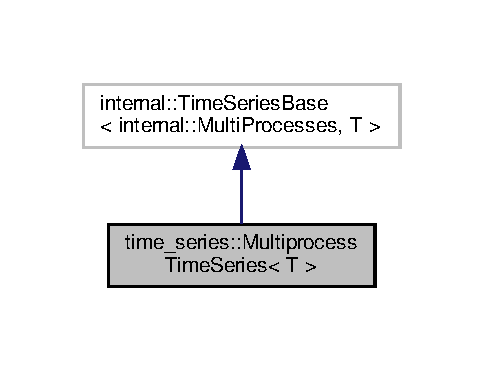
\includegraphics[width=265pt]{classtime__series_1_1MultiprocessTimeSeries__inherit__graph}
\end{center}
\end{figure}


Collaboration diagram for time\+\_\+series\+:\+:Multiprocess\+Time\+Series$<$ T $>$\+:
\nopagebreak
\begin{figure}[H]
\begin{center}
\leavevmode
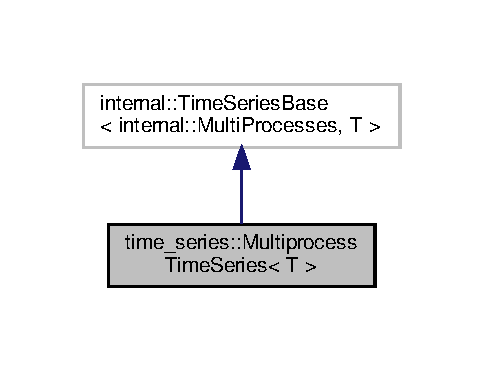
\includegraphics[width=265pt]{classtime__series_1_1MultiprocessTimeSeries__coll__graph}
\end{center}
\end{figure}
\subsection*{Public Member Functions}
\begin{DoxyCompactItemize}
\item 
\hyperlink{classtime__series_1_1MultiprocessTimeSeries_a118890497b42365a56221c66edbb478e}{Multiprocess\+Time\+Series} (std\+::string segment\+\_\+id, size\+\_\+t \hyperlink{classtime__series_1_1internal_1_1TimeSeriesBase_aee1bf636a094a3068f9de731688c3972}{max\+\_\+length}, bool leader=true, Index start\+\_\+timeindex=0)
\begin{DoxyCompactList}\small\item\em create a new instance pointing to the specified shared memory segment \end{DoxyCompactList}\end{DoxyCompactItemize}
\subsection*{Protected Member Functions}
\begin{DoxyCompactItemize}
\item 
\mbox{\Hypertarget{classtime__series_1_1MultiprocessTimeSeries_a44445322f664019684a02caa31639c14}\label{classtime__series_1_1MultiprocessTimeSeries_a44445322f664019684a02caa31639c14}} 
void {\bfseries read\+\_\+indexes} ()
\item 
\mbox{\Hypertarget{classtime__series_1_1MultiprocessTimeSeries_abc59736f908b8e3f4e6881607e2253a7}\label{classtime__series_1_1MultiprocessTimeSeries_abc59736f908b8e3f4e6881607e2253a7}} 
void {\bfseries write\+\_\+indexes} ()
\end{DoxyCompactItemize}
\subsection*{Protected Attributes}
\begin{DoxyCompactItemize}
\item 
\mbox{\Hypertarget{classtime__series_1_1MultiprocessTimeSeries_a0ae05ba33e9f73f839e2229677062518}\label{classtime__series_1_1MultiprocessTimeSeries_a0ae05ba33e9f73f839e2229677062518}} 
shared\+\_\+memory\+::array$<$ Index $>$ {\bfseries indexes\+\_\+}
\end{DoxyCompactItemize}


\subsection{Detailed Description}
\subsubsection*{template$<$typename T = int$>$\newline
class time\+\_\+series\+::\+Multiprocess\+Time\+Series$<$ T $>$}

Multiprocess Time Series. 

Several instances hosted by different processes, if pointing to the same shared memory segment (as specified by the segment\+\_\+id), may read/write from the same underlying time series. 

\subsection{Constructor \& Destructor Documentation}
\mbox{\Hypertarget{classtime__series_1_1MultiprocessTimeSeries_a118890497b42365a56221c66edbb478e}\label{classtime__series_1_1MultiprocessTimeSeries_a118890497b42365a56221c66edbb478e}} 
\index{time\+\_\+series\+::\+Multiprocess\+Time\+Series@{time\+\_\+series\+::\+Multiprocess\+Time\+Series}!Multiprocess\+Time\+Series@{Multiprocess\+Time\+Series}}
\index{Multiprocess\+Time\+Series@{Multiprocess\+Time\+Series}!time\+\_\+series\+::\+Multiprocess\+Time\+Series@{time\+\_\+series\+::\+Multiprocess\+Time\+Series}}
\subsubsection{\texorpdfstring{Multiprocess\+Time\+Series()}{MultiprocessTimeSeries()}}
{\footnotesize\ttfamily template$<$typename T  = int$>$ \\
\hyperlink{classtime__series_1_1MultiprocessTimeSeries}{time\+\_\+series\+::\+Multiprocess\+Time\+Series}$<$ T $>$\+::\hyperlink{classtime__series_1_1MultiprocessTimeSeries}{Multiprocess\+Time\+Series} (\begin{DoxyParamCaption}\item[{std\+::string}]{segment\+\_\+id,  }\item[{size\+\_\+t}]{max\+\_\+length,  }\item[{bool}]{leader = {\ttfamily true},  }\item[{Index}]{start\+\_\+timeindex = {\ttfamily 0} }\end{DoxyParamCaption})\hspace{0.3cm}{\ttfamily [inline]}}



create a new instance pointing to the specified shared memory segment 


\begin{DoxyParams}{Parameters}
{\em segment\+\_\+id} & the id of the segment to point to \\
\hline
{\em max\+\_\+length} & max number of elements in the time series \\
\hline
{\em leader} & if true, the shared memory segment will initialize the shared time series, and wiped the related shared memory on destruction. Instantiating a first \hyperlink{classtime__series_1_1MultiprocessTimeSeries}{Multiprocess\+Time\+Series} with leader set to false will result in undefined behavior. When the leader instance is destroyed, other instances are pointing to the shared segment may crash or hang. \\
\hline
\end{DoxyParams}


The documentation for this class was generated from the following file\+:\begin{DoxyCompactItemize}
\item 
include/time\+\_\+series/multiprocess\+\_\+time\+\_\+series.\+hpp\end{DoxyCompactItemize}

\hypertarget{classtime__series_1_1TimeSeries}{}\section{time\+\_\+series\+:\+:Time\+Series$<$ T $>$ Class Template Reference}
\label{classtime__series_1_1TimeSeries}\index{time\+\_\+series\+::\+Time\+Series$<$ T $>$@{time\+\_\+series\+::\+Time\+Series$<$ T $>$}}


Threadsafe time series.  




{\ttfamily \#include $<$time\+\_\+series.\+hpp$>$}



Inheritance diagram for time\+\_\+series\+:\+:Time\+Series$<$ T $>$\+:
\nopagebreak
\begin{figure}[H]
\begin{center}
\leavevmode
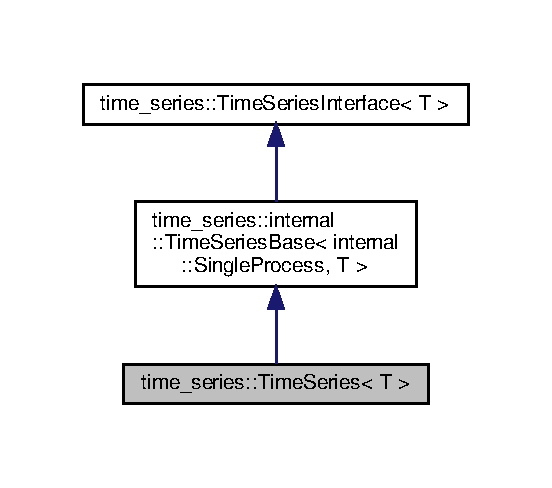
\includegraphics[width=265pt]{classtime__series_1_1TimeSeries__inherit__graph}
\end{center}
\end{figure}


Collaboration diagram for time\+\_\+series\+:\+:Time\+Series$<$ T $>$\+:
\nopagebreak
\begin{figure}[H]
\begin{center}
\leavevmode
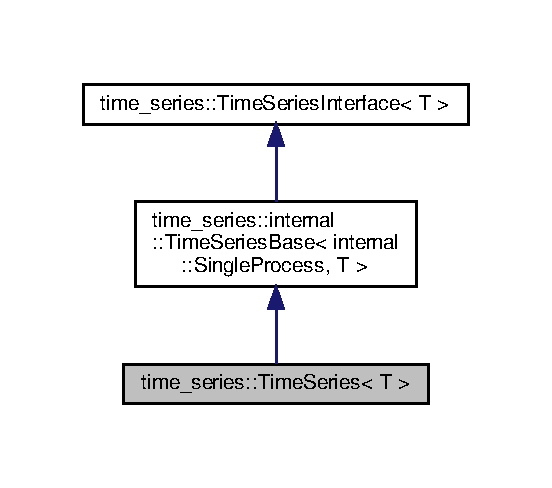
\includegraphics[width=265pt]{classtime__series_1_1TimeSeries__coll__graph}
\end{center}
\end{figure}
\subsection*{Public Member Functions}
\begin{DoxyCompactItemize}
\item 
{\bfseries Time\+Series} (size\+\_\+t \hyperlink{classtime__series_1_1internal_1_1TimeSeriesBase_aee1bf636a094a3068f9de731688c3972}{max\+\_\+length}, Index start\+\_\+timeindex=0)\hypertarget{classtime__series_1_1TimeSeries_abd15b59569dc3dca7d1b848a0867a117}{}\label{classtime__series_1_1TimeSeries_abd15b59569dc3dca7d1b848a0867a117}

\end{DoxyCompactItemize}
\subsection*{Protected Member Functions}
\begin{DoxyCompactItemize}
\item 
void {\bfseries read\+\_\+indexes} ()\hypertarget{classtime__series_1_1TimeSeries_acbd2aa3299e5c62811df429896791767}{}\label{classtime__series_1_1TimeSeries_acbd2aa3299e5c62811df429896791767}

\item 
void {\bfseries write\+\_\+indexes} ()\hypertarget{classtime__series_1_1TimeSeries_a0fdedf27b55bbf78eed4d35f82cf3ace}{}\label{classtime__series_1_1TimeSeries_a0fdedf27b55bbf78eed4d35f82cf3ace}

\end{DoxyCompactItemize}
\subsection*{Additional Inherited Members}


\subsection{Detailed Description}
\subsubsection*{template$<$typename T = int$>$\\*
class time\+\_\+series\+::\+Time\+Series$<$ T $>$}

Threadsafe time series. 

The documentation for this class was generated from the following file\+:\begin{DoxyCompactItemize}
\item 
include/time\+\_\+series/\hyperlink{time__series_8hpp}{time\+\_\+series.\+hpp}\end{DoxyCompactItemize}

\hypertarget{classtime__series_1_1TimeSeriesInterface}{}\section{time\+\_\+series\+:\+:Time\+Series\+Interface$<$ T $>$ Class Template Reference}
\label{classtime__series_1_1TimeSeriesInterface}\index{time\+\_\+series\+::\+Time\+Series\+Interface$<$ T $>$@{time\+\_\+series\+::\+Time\+Series\+Interface$<$ T $>$}}


Interface for time series.  




{\ttfamily \#include $<$interface.\+hpp$>$}



Inheritance diagram for time\+\_\+series\+:\+:Time\+Series\+Interface$<$ T $>$\+:
\nopagebreak
\begin{figure}[H]
\begin{center}
\leavevmode
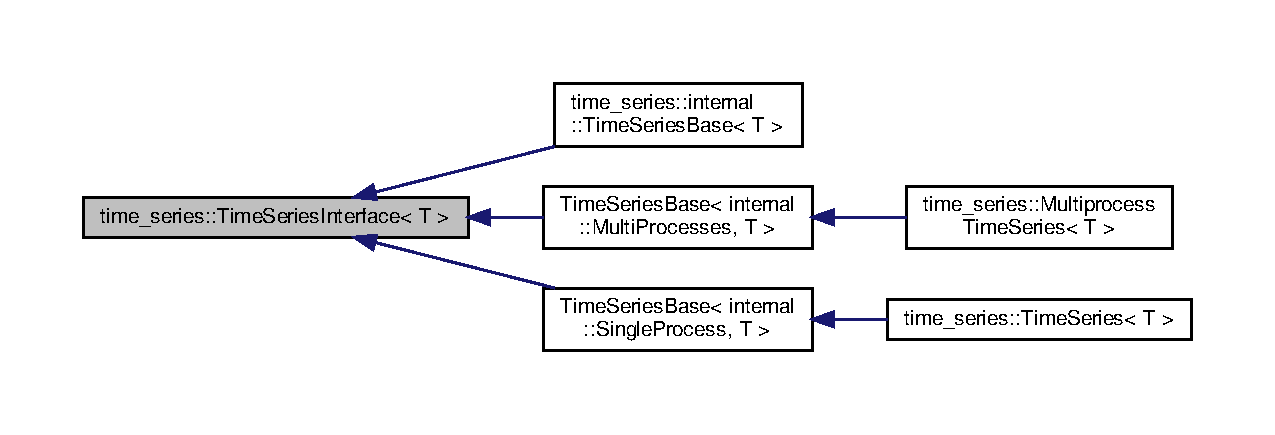
\includegraphics[width=350pt]{classtime__series_1_1TimeSeriesInterface__inherit__graph}
\end{center}
\end{figure}
\subsection*{Public Member Functions}
\begin{DoxyCompactItemize}
\item 
\mbox{\Hypertarget{classtime__series_1_1TimeSeriesInterface_a19127d715b58f95c0e2581576fe80f18}\label{classtime__series_1_1TimeSeriesInterface_a19127d715b58f95c0e2581576fe80f18}} 
virtual Index \hyperlink{classtime__series_1_1TimeSeriesInterface_a19127d715b58f95c0e2581576fe80f18}{newest\+\_\+timeindex} (bool wait=true)=0
\begin{DoxyCompactList}\small\item\em returns $ newest $ index. If argument wait is true, waits if the time\+\_\+series is empty. If argument wait is false and the time series is empty, returns time\+\_\+series\+::\+E\+M\+P\+TY immediately. \end{DoxyCompactList}\item 
\mbox{\Hypertarget{classtime__series_1_1TimeSeriesInterface_a46cf7fc73adfcc400fbf40c22aa7268f}\label{classtime__series_1_1TimeSeriesInterface_a46cf7fc73adfcc400fbf40c22aa7268f}} 
virtual Index \hyperlink{classtime__series_1_1TimeSeriesInterface_a46cf7fc73adfcc400fbf40c22aa7268f}{count\+\_\+appended\+\_\+elements} ()=0
\begin{DoxyCompactList}\small\item\em returns the number of element that has been contained in the queue, i.\+e. the number of elements that have been added from the start. \end{DoxyCompactList}\item 
\mbox{\Hypertarget{classtime__series_1_1TimeSeriesInterface_a3a68de9ecf8bfeb6c05ea89386537307}\label{classtime__series_1_1TimeSeriesInterface_a3a68de9ecf8bfeb6c05ea89386537307}} 
virtual Index \hyperlink{classtime__series_1_1TimeSeriesInterface_a3a68de9ecf8bfeb6c05ea89386537307}{oldest\+\_\+timeindex} (bool wait=true)=0
\begin{DoxyCompactList}\small\item\em returns $ oldest $. waits if the time\+\_\+series is empty. If argument wait is false and the time series is empty, returns time\+\_\+series\+::\+E\+M\+P\+TY immediately. \end{DoxyCompactList}\item 
\mbox{\Hypertarget{classtime__series_1_1TimeSeriesInterface_ad3b66b6b5f0f763d440731c50e41b4cb}\label{classtime__series_1_1TimeSeriesInterface_ad3b66b6b5f0f763d440731c50e41b4cb}} 
virtual T \hyperlink{classtime__series_1_1TimeSeriesInterface_ad3b66b6b5f0f763d440731c50e41b4cb}{newest\+\_\+element} ()=0
\begin{DoxyCompactList}\small\item\em returns $ X_{newest} $. waits if the time\+\_\+series is empty. \end{DoxyCompactList}\item 
\mbox{\Hypertarget{classtime__series_1_1TimeSeriesInterface_a3149f64961e08315eb06798d0f075333}\label{classtime__series_1_1TimeSeriesInterface_a3149f64961e08315eb06798d0f075333}} 
virtual T \hyperlink{classtime__series_1_1TimeSeriesInterface_a3149f64961e08315eb06798d0f075333}{operator\mbox{[}$\,$\mbox{]}} (const Index \&timeindex)=0
\begin{DoxyCompactList}\small\item\em returns $ X_{timeindex} $. waits if the time\+\_\+series is empty or if $timeindex > newest $. \end{DoxyCompactList}\item 
\mbox{\Hypertarget{classtime__series_1_1TimeSeriesInterface_aaeb745c8c13170a645b25170f0b035f1}\label{classtime__series_1_1TimeSeriesInterface_aaeb745c8c13170a645b25170f0b035f1}} 
virtual Timestamp \hyperlink{classtime__series_1_1TimeSeriesInterface_aaeb745c8c13170a645b25170f0b035f1}{timestamp\+\_\+ms} (const Index \&timeindex)=0
\begin{DoxyCompactList}\small\item\em returns the time in miliseconds when $ X_{timeindex} $ was appended. Waits if the time\+\_\+series is empty or if $timeindex > newest $. \end{DoxyCompactList}\item 
\mbox{\Hypertarget{classtime__series_1_1TimeSeriesInterface_acfb468e6e1766fe4b566189d3b888e4d}\label{classtime__series_1_1TimeSeriesInterface_acfb468e6e1766fe4b566189d3b888e4d}} 
virtual Timestamp \hyperlink{classtime__series_1_1TimeSeriesInterface_acfb468e6e1766fe4b566189d3b888e4d}{timestamp\+\_\+s} (const Index \&timeindex)=0
\begin{DoxyCompactList}\small\item\em returns the time in seconds when $ X_{timeindex} $ was appended. Waits if the time\+\_\+series is empty or if $timeindex > newest $. \end{DoxyCompactList}\item 
\mbox{\Hypertarget{classtime__series_1_1TimeSeriesInterface_aa09c55259a1f34491b5ecdd1505ffdbf}\label{classtime__series_1_1TimeSeriesInterface_aa09c55259a1f34491b5ecdd1505ffdbf}} 
virtual bool \hyperlink{classtime__series_1_1TimeSeriesInterface_aa09c55259a1f34491b5ecdd1505ffdbf}{wait\+\_\+for\+\_\+timeindex} (const Index \&timeindex, const double \&max\+\_\+duration\+\_\+s=std\+::numeric\+\_\+limits$<$ double $>$\+::quiet\+\_\+\+NaN())=0
\begin{DoxyCompactList}\small\item\em Wait until the defined time index is reached. If the input time is below the oldest time index that have been registered read an exception is return. \end{DoxyCompactList}\item 
\mbox{\Hypertarget{classtime__series_1_1TimeSeriesInterface_a90f6ed15d82006dbc7ef7783d9f6ff7a}\label{classtime__series_1_1TimeSeriesInterface_a90f6ed15d82006dbc7ef7783d9f6ff7a}} 
virtual std\+::size\+\_\+t \hyperlink{classtime__series_1_1TimeSeriesInterface_a90f6ed15d82006dbc7ef7783d9f6ff7a}{length} ()=0
\begin{DoxyCompactList}\small\item\em returns the length of the time\+\_\+series, i.\+e. $0$ if it is empty, otherwise $newest - oldest +1 $. \end{DoxyCompactList}\item 
virtual std\+::size\+\_\+t \hyperlink{classtime__series_1_1TimeSeriesInterface_aded8927e82c060aa3367f17dfd59a8ec}{max\+\_\+length} ()=0
\begin{DoxyCompactList}\small\item\em returns the maximum length of the time serie. \end{DoxyCompactList}\item 
\mbox{\Hypertarget{classtime__series_1_1TimeSeriesInterface_a2758b463ea41393a24ea37ccd0f5feb4}\label{classtime__series_1_1TimeSeriesInterface_a2758b463ea41393a24ea37ccd0f5feb4}} 
virtual bool \hyperlink{classtime__series_1_1TimeSeriesInterface_a2758b463ea41393a24ea37ccd0f5feb4}{has\+\_\+changed\+\_\+since\+\_\+tag} ()=0
\begin{DoxyCompactList}\small\item\em returns boolean indicating whether new elements have been appended since the last time the \hyperlink{classtime__series_1_1TimeSeriesInterface_a34e881c9496901127baf1d907d7399ac}{tag()} function was called. \end{DoxyCompactList}\item 
\mbox{\Hypertarget{classtime__series_1_1TimeSeriesInterface_a34e881c9496901127baf1d907d7399ac}\label{classtime__series_1_1TimeSeriesInterface_a34e881c9496901127baf1d907d7399ac}} 
virtual void \hyperlink{classtime__series_1_1TimeSeriesInterface_a34e881c9496901127baf1d907d7399ac}{tag} (const Index \&timeindex)=0
\begin{DoxyCompactList}\small\item\em tags the current time\+\_\+series, can later be used to check whether new elements have been added \end{DoxyCompactList}\item 
\mbox{\Hypertarget{classtime__series_1_1TimeSeriesInterface_aa71ab509ac29c5da681aee9dbf65f2d8}\label{classtime__series_1_1TimeSeriesInterface_aa71ab509ac29c5da681aee9dbf65f2d8}} 
virtual Index \hyperlink{classtime__series_1_1TimeSeriesInterface_aa71ab509ac29c5da681aee9dbf65f2d8}{tagged\+\_\+timeindex} ()=0
\begin{DoxyCompactList}\small\item\em returns the index at which the time series has been tagged. Returns the newest timeindex if the time series has never been tagged. \end{DoxyCompactList}\item 
\mbox{\Hypertarget{classtime__series_1_1TimeSeriesInterface_a0782c522287cf041fc253529b61041f9}\label{classtime__series_1_1TimeSeriesInterface_a0782c522287cf041fc253529b61041f9}} 
virtual void \hyperlink{classtime__series_1_1TimeSeriesInterface_a0782c522287cf041fc253529b61041f9}{append} (const T \&element)=0
\begin{DoxyCompactList}\small\item\em appends a new element to the time\+\_\+series, e.\+g. we go from $ X_{1:10} $ to $ X_{1:11} $ (where $ X_{11}=$ element). if the time\+\_\+series length is already equal to its max\+\_\+length, then the oldest element is discarded, e.\+g. for a max\+\_\+length = 10 we would go from $ X_{1:10} $ to $ X_{2:11} $. \end{DoxyCompactList}\item 
\mbox{\Hypertarget{classtime__series_1_1TimeSeriesInterface_a932e891f3f41781af4282ada18f05d31}\label{classtime__series_1_1TimeSeriesInterface_a932e891f3f41781af4282ada18f05d31}} 
virtual bool \hyperlink{classtime__series_1_1TimeSeriesInterface_a932e891f3f41781af4282ada18f05d31}{is\+\_\+empty} ()=0
\begin{DoxyCompactList}\small\item\em returns true if no element has ever been appended to the time series. \end{DoxyCompactList}\end{DoxyCompactItemize}


\subsection{Detailed Description}
\subsubsection*{template$<$typename T$>$\newline
class time\+\_\+series\+::\+Time\+Series\+Interface$<$ T $>$}

Interface for time series. 

A time\+\_\+series implements $ X_{{oldest}:{newest}} $ which can safely be accessed from either multiple threads or multiple processes.

this object has the following properties\+:
\begin{DoxyItemize}
\item an oldest timeindex $ oldest$,
\item a newest timeindex $ newest $,
\item a value $ X_i $ for each $ i \in \{oldest, oldest + 1 , ..., newest\} $,
\item a length $length$
\item and a maximum length $maxlength$ 
\end{DoxyItemize}

\subsection{Member Function Documentation}
\mbox{\Hypertarget{classtime__series_1_1TimeSeriesInterface_aded8927e82c060aa3367f17dfd59a8ec}\label{classtime__series_1_1TimeSeriesInterface_aded8927e82c060aa3367f17dfd59a8ec}} 
\index{time\+\_\+series\+::\+Time\+Series\+Interface@{time\+\_\+series\+::\+Time\+Series\+Interface}!max\+\_\+length@{max\+\_\+length}}
\index{max\+\_\+length@{max\+\_\+length}!time\+\_\+series\+::\+Time\+Series\+Interface@{time\+\_\+series\+::\+Time\+Series\+Interface}}
\subsubsection{\texorpdfstring{max\+\_\+length()}{max\_length()}}
{\footnotesize\ttfamily template$<$typename T $>$ \\
virtual std\+::size\+\_\+t \hyperlink{classtime__series_1_1TimeSeriesInterface}{time\+\_\+series\+::\+Time\+Series\+Interface}$<$ T $>$\+::max\+\_\+length (\begin{DoxyParamCaption}{ }\end{DoxyParamCaption})\hspace{0.3cm}{\ttfamily [pure virtual]}}



returns the maximum length of the time serie. 

\begin{DoxyReturn}{Returns}
std\+::size\+\_\+t 
\end{DoxyReturn}


Implemented in \hyperlink{classtime__series_1_1internal_1_1TimeSeriesBase_aee1bf636a094a3068f9de731688c3972}{time\+\_\+series\+::internal\+::\+Time\+Series\+Base$<$ P, T $>$}, \hyperlink{classtime__series_1_1internal_1_1TimeSeriesBase_aee1bf636a094a3068f9de731688c3972}{time\+\_\+series\+::internal\+::\+Time\+Series\+Base$<$ internal\+::\+Single\+Process, T $>$}, and \hyperlink{classtime__series_1_1internal_1_1TimeSeriesBase_aee1bf636a094a3068f9de731688c3972}{time\+\_\+series\+::internal\+::\+Time\+Series\+Base$<$ internal\+::\+Multi\+Processes, T $>$}.



The documentation for this class was generated from the following file\+:\begin{DoxyCompactItemize}
\item 
include/time\+\_\+series/\hyperlink{interface_8hpp}{interface.\+hpp}\end{DoxyCompactItemize}

\chapter{File Documentation}
\hypertarget{demo__multiprocess__read_8cpp}{}\section{demos/demo\+\_\+multiprocess\+\_\+read.cpp File Reference}
\label{demo__multiprocess__read_8cpp}\index{demos/demo\+\_\+multiprocess\+\_\+read.\+cpp@{demos/demo\+\_\+multiprocess\+\_\+read.\+cpp}}


Read data from a shared timed series. This demo does nothing until demo\+\_\+multiprocess\+\_\+write is started. ctrl+c for exit.  


{\ttfamily \#include \char`\"{}shared\+\_\+memory/demos/item.\+hpp\char`\"{}}\newline
{\ttfamily \#include \char`\"{}time\+\_\+series/multiprocess\+\_\+time\+\_\+series.\+hpp\char`\"{}}\newline
Include dependency graph for demo\+\_\+multiprocess\+\_\+read.\+cpp\+:
\nopagebreak
\begin{figure}[H]
\begin{center}
\leavevmode
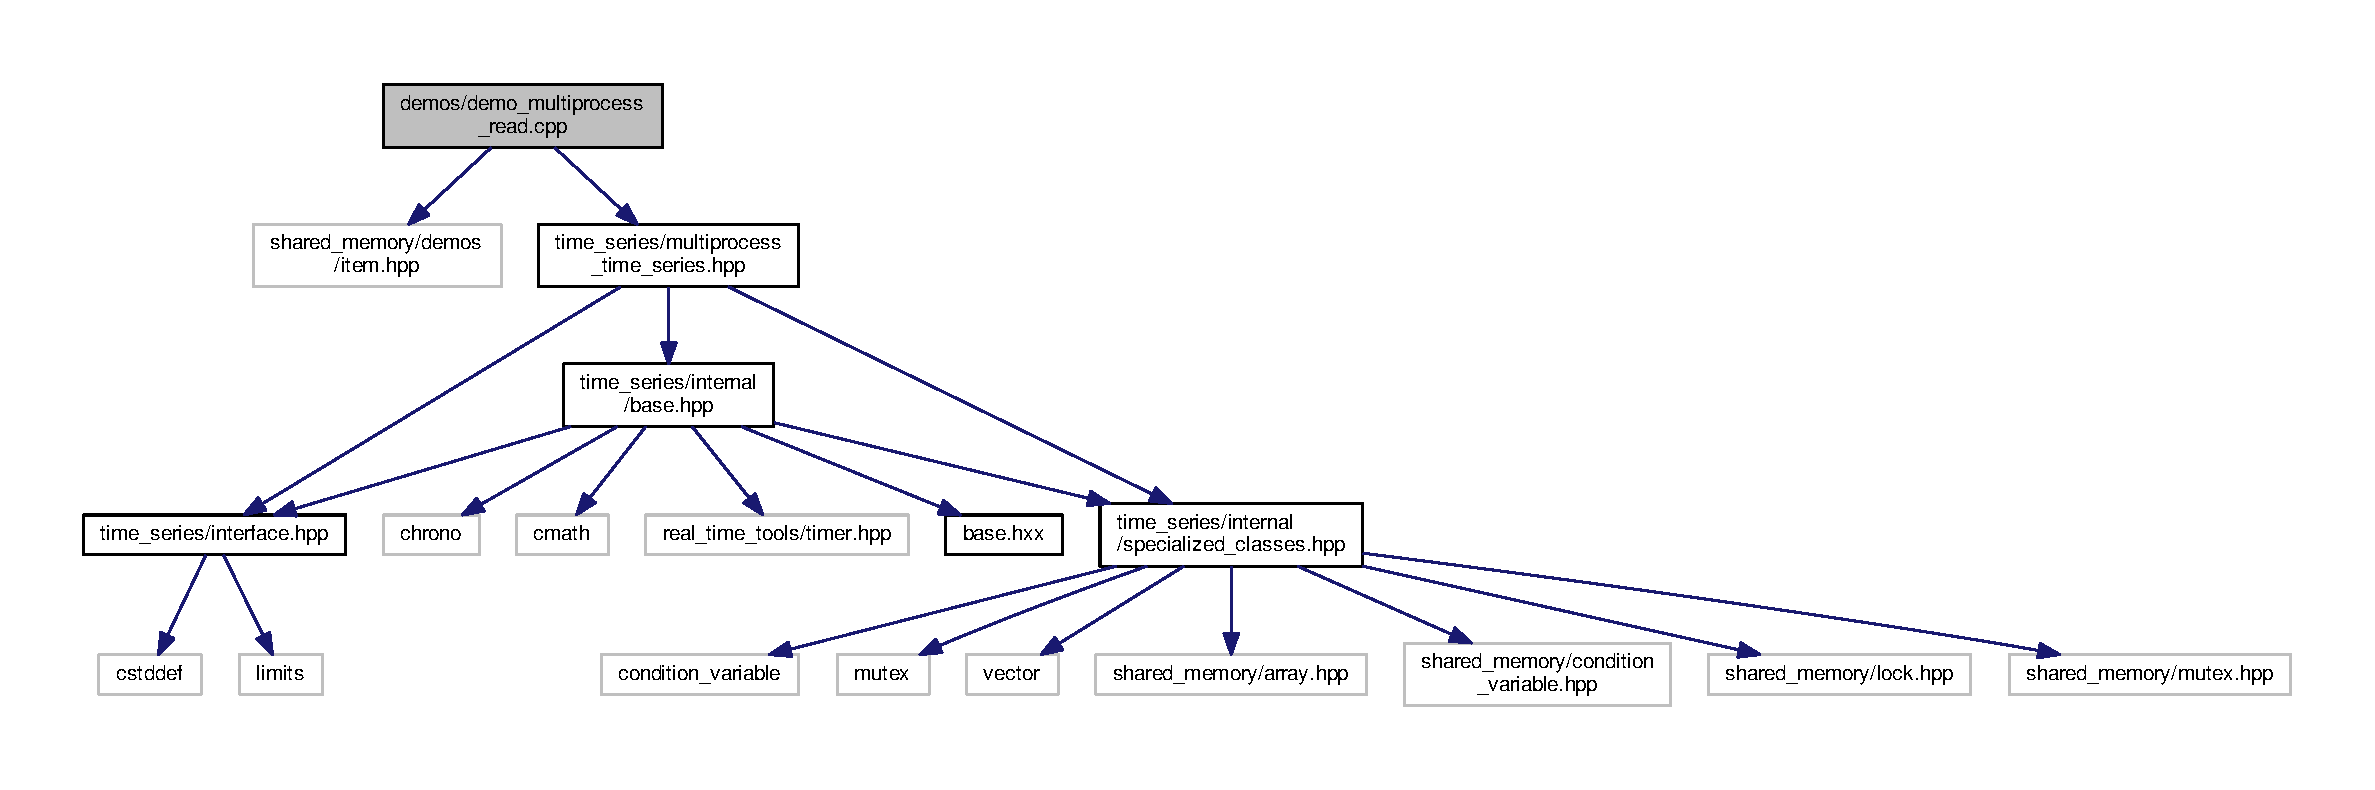
\includegraphics[width=350pt]{demo__multiprocess__read_8cpp__incl}
\end{center}
\end{figure}
\subsection*{Macros}
\begin{DoxyCompactItemize}
\item 
\mbox{\Hypertarget{demo__multiprocess__read_8cpp_aa2341624eba49f3cdec3d9656b97cd79}\label{demo__multiprocess__read_8cpp_aa2341624eba49f3cdec3d9656b97cd79}} 
\#define {\bfseries S\+E\+G\+M\+E\+N\+T\+\_\+\+ID}~\char`\"{}demo\+\_\+time\+\_\+series\+\_\+multiprocess\char`\"{}
\item 
\mbox{\Hypertarget{demo__multiprocess__read_8cpp_ad279f2fa0f02868c901c0d29d41af6d6}\label{demo__multiprocess__read_8cpp_ad279f2fa0f02868c901c0d29d41af6d6}} 
\#define {\bfseries T\+I\+M\+E\+S\+E\+R\+I\+E\+S\+\_\+\+S\+I\+ZE}~100
\end{DoxyCompactItemize}
\subsection*{Typedefs}
\begin{DoxyCompactItemize}
\item 
\mbox{\Hypertarget{demo__multiprocess__read_8cpp_a80d365cd1fbfb7d75ecfab72e362b360}\label{demo__multiprocess__read_8cpp_a80d365cd1fbfb7d75ecfab72e362b360}} 
typedef \hyperlink{classtime__series_1_1MultiprocessTimeSeries}{time\+\_\+series\+::\+Multiprocess\+Time\+Series}$<$ shared\+\_\+memory\+::\+Item$<$ 10 $>$ $>$ {\bfseries Time\+Series}
\end{DoxyCompactItemize}
\subsection*{Functions}
\begin{DoxyCompactItemize}
\item 
\mbox{\Hypertarget{demo__multiprocess__read_8cpp_a13a43e6d814de94978c515cb084873b1}\label{demo__multiprocess__read_8cpp_a13a43e6d814de94978c515cb084873b1}} 
void \hyperlink{demo__multiprocess__read_8cpp_a13a43e6d814de94978c515cb084873b1}{run} ()
\begin{DoxyCompactList}\small\item\em read (and print) items written by demo\+\_\+multiprocess\+\_\+write \end{DoxyCompactList}\item 
\mbox{\Hypertarget{demo__multiprocess__read_8cpp_ae66f6b31b5ad750f1fe042a706a4e3d4}\label{demo__multiprocess__read_8cpp_ae66f6b31b5ad750f1fe042a706a4e3d4}} 
int {\bfseries main} ()
\end{DoxyCompactItemize}


\subsection{Detailed Description}
Read data from a shared timed series. This demo does nothing until demo\+\_\+multiprocess\+\_\+write is started. ctrl+c for exit. 

\begin{DoxyAuthor}{Author}
Vincent Berenz 
\end{DoxyAuthor}
\begin{DoxyCopyright}{Copyright}
Copyright (c) 2019, Max Planck Gesellschaft. 
\end{DoxyCopyright}

\hypertarget{demo__multiprocess__write_8cpp}{}\section{demos/demo\+\_\+multiprocess\+\_\+write.cpp File Reference}
\label{demo__multiprocess__write_8cpp}\index{demos/demo\+\_\+multiprocess\+\_\+write.\+cpp@{demos/demo\+\_\+multiprocess\+\_\+write.\+cpp}}


Write data into a shared timed series. The demo demo\+\_\+multiprocess\+\_\+read is expected to be already running when this demo is started. Infinite hanging may occur otherwhise.  


{\ttfamily \#include \char`\"{}shared\+\_\+memory/demos/item.\+hpp\char`\"{}}\\*
{\ttfamily \#include \char`\"{}time\+\_\+series/multiprocess\+\_\+time\+\_\+series.\+hpp\char`\"{}}\\*
Include dependency graph for demo\+\_\+multiprocess\+\_\+write.\+cpp\+:
\nopagebreak
\begin{figure}[H]
\begin{center}
\leavevmode
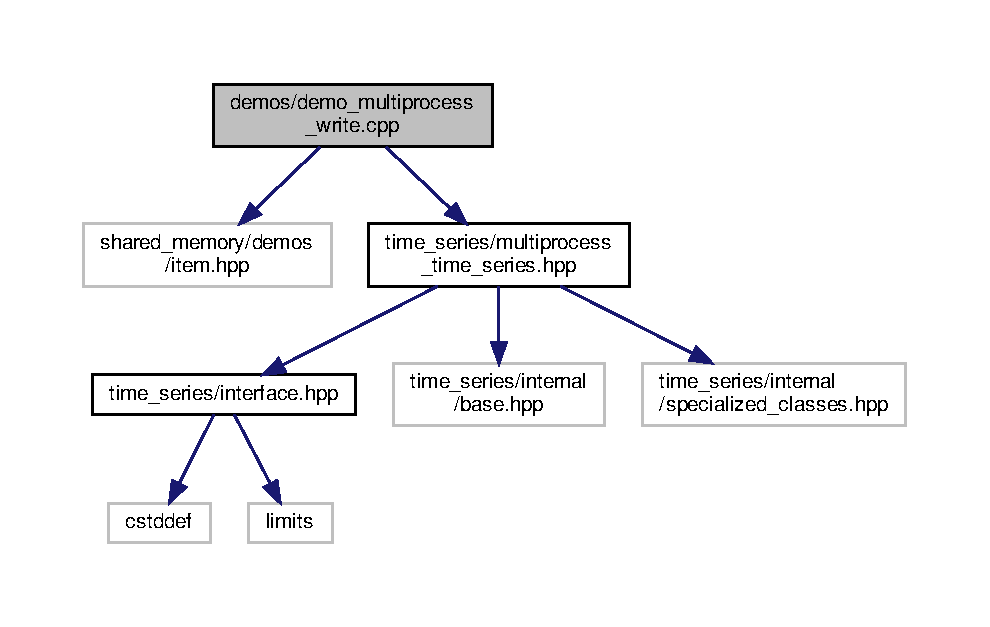
\includegraphics[width=350pt]{demo__multiprocess__write_8cpp__incl}
\end{center}
\end{figure}
\subsection*{Macros}
\begin{DoxyCompactItemize}
\item 
\#define {\bfseries S\+E\+G\+M\+E\+N\+T\+\_\+\+ID}~\char`\"{}demo\+\_\+time\+\_\+series\+\_\+multiprocess\char`\"{}\hypertarget{demo__multiprocess__write_8cpp_aa2341624eba49f3cdec3d9656b97cd79}{}\label{demo__multiprocess__write_8cpp_aa2341624eba49f3cdec3d9656b97cd79}

\item 
\#define {\bfseries T\+I\+M\+E\+S\+E\+R\+I\+E\+S\+\_\+\+S\+I\+ZE}~100\hypertarget{demo__multiprocess__write_8cpp_ad279f2fa0f02868c901c0d29d41af6d6}{}\label{demo__multiprocess__write_8cpp_ad279f2fa0f02868c901c0d29d41af6d6}

\end{DoxyCompactItemize}
\subsection*{Typedefs}
\begin{DoxyCompactItemize}
\item 
typedef \hyperlink{classtime__series_1_1MultiprocessTimeSeries}{time\+\_\+series\+::\+Multiprocess\+Time\+Series}$<$ shared\+\_\+memory\+::\+Item$<$ 10 $>$ $>$ {\bfseries T\+I\+M\+E\+S\+E\+R\+I\+ES}\hypertarget{demo__multiprocess__write_8cpp_a6663308ba00701256d3afe22992c48cf}{}\label{demo__multiprocess__write_8cpp_a6663308ba00701256d3afe22992c48cf}

\end{DoxyCompactItemize}
\subsection*{Functions}
\begin{DoxyCompactItemize}
\item 
void {\bfseries run} ()\hypertarget{demo__multiprocess__write_8cpp_a13a43e6d814de94978c515cb084873b1}{}\label{demo__multiprocess__write_8cpp_a13a43e6d814de94978c515cb084873b1}

\item 
int {\bfseries main} ()\hypertarget{demo__multiprocess__write_8cpp_ae66f6b31b5ad750f1fe042a706a4e3d4}{}\label{demo__multiprocess__write_8cpp_ae66f6b31b5ad750f1fe042a706a4e3d4}

\end{DoxyCompactItemize}


\subsection{Detailed Description}
Write data into a shared timed series. The demo demo\+\_\+multiprocess\+\_\+read is expected to be already running when this demo is started. Infinite hanging may occur otherwhise. 

\begin{DoxyAuthor}{Author}
Vincent Berenz 
\end{DoxyAuthor}
\begin{DoxyCopyright}{Copyright}
Copyright (c) 2019, Max Planck Gesellschaft. 
\end{DoxyCopyright}

\hypertarget{demo__time__series_8cpp}{}\section{demos/demo\+\_\+time\+\_\+series.cpp File Reference}
\label{demo__time__series_8cpp}\index{demos/demo\+\_\+time\+\_\+series.\+cpp@{demos/demo\+\_\+time\+\_\+series.\+cpp}}


basic usage of time series  


{\ttfamily \#include \char`\"{}real\+\_\+time\+\_\+tools/thread.\+hpp\char`\"{}}\newline
{\ttfamily \#include \char`\"{}time\+\_\+series/time\+\_\+series.\+hpp\char`\"{}}\newline
Include dependency graph for demo\+\_\+time\+\_\+series.\+cpp\+:
\nopagebreak
\begin{figure}[H]
\begin{center}
\leavevmode
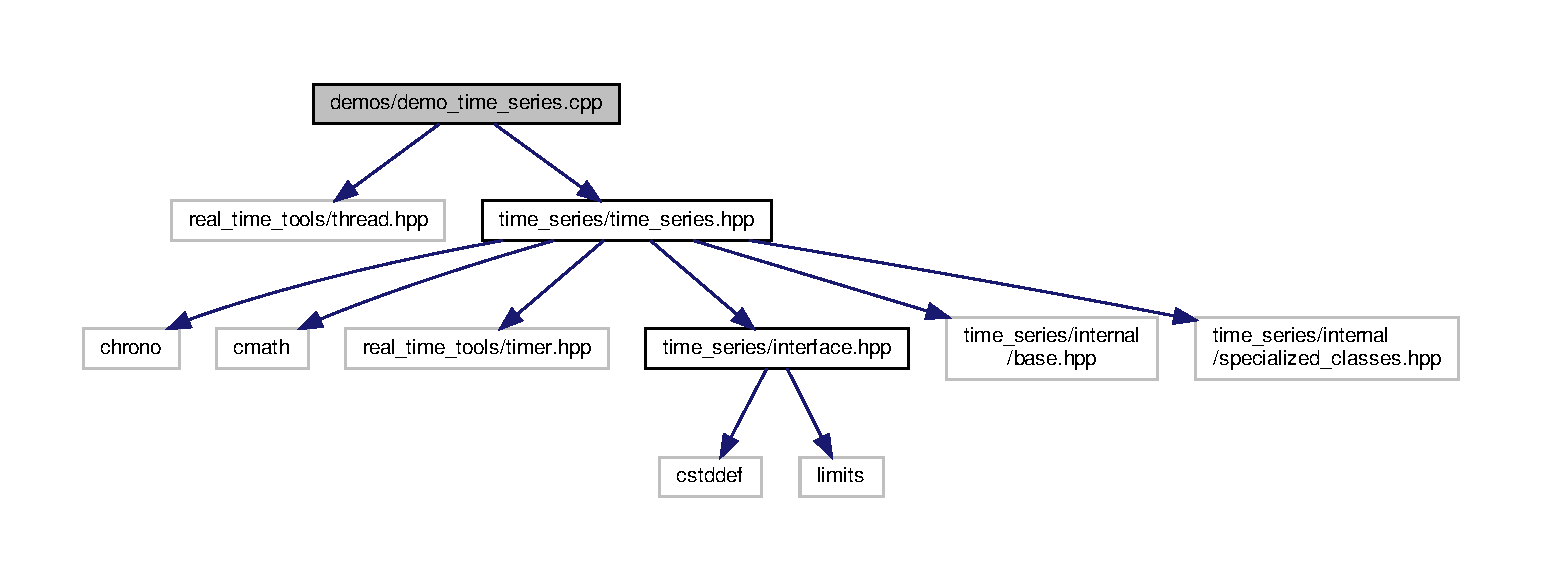
\includegraphics[width=350pt]{demo__time__series_8cpp__incl}
\end{center}
\end{figure}
\subsection*{Functions}
\begin{DoxyCompactItemize}
\item 
\mbox{\Hypertarget{demo__time__series_8cpp_a518842da1ba4ef4ba8c7f57fd9731cfc}\label{demo__time__series_8cpp_a518842da1ba4ef4ba8c7f57fd9731cfc}} 
void $\ast$ \hyperlink{demo__time__series_8cpp_a518842da1ba4ef4ba8c7f57fd9731cfc}{producer} (void $\ast$args)
\begin{DoxyCompactList}\small\item\em Write values to the time series. \end{DoxyCompactList}\item 
\mbox{\Hypertarget{demo__time__series_8cpp_a13a43e6d814de94978c515cb084873b1}\label{demo__time__series_8cpp_a13a43e6d814de94978c515cb084873b1}} 
void \hyperlink{demo__time__series_8cpp_a13a43e6d814de94978c515cb084873b1}{run} ()
\begin{DoxyCompactList}\small\item\em Read and display the values from the time series. \end{DoxyCompactList}\item 
\mbox{\Hypertarget{demo__time__series_8cpp_ae66f6b31b5ad750f1fe042a706a4e3d4}\label{demo__time__series_8cpp_ae66f6b31b5ad750f1fe042a706a4e3d4}} 
int {\bfseries main} ()
\end{DoxyCompactItemize}
\subsection*{Variables}
\begin{DoxyCompactItemize}
\item 
\mbox{\Hypertarget{demo__time__series_8cpp_a82d33897ce200eadf132e93031f0e595}\label{demo__time__series_8cpp_a82d33897ce200eadf132e93031f0e595}} 
bool {\bfseries g\+\_\+running} = true
\end{DoxyCompactItemize}


\subsection{Detailed Description}
basic usage of time series 

\begin{DoxyAuthor}{Author}
Vincent Berenz 
\end{DoxyAuthor}
\begin{DoxyCopyright}{Copyright}
Copyright (c) 2019, Max Planck Gesellschaft. 
\end{DoxyCopyright}

\hypertarget{interface_8hpp}{}\section{include/time\+\_\+series/interface.hpp File Reference}
\label{interface_8hpp}\index{include/time\+\_\+series/interface.\+hpp@{include/time\+\_\+series/interface.\+hpp}}
{\ttfamily \#include $<$cstddef$>$}\newline
{\ttfamily \#include $<$limits$>$}\newline
Include dependency graph for interface.\+hpp\+:
\nopagebreak
\begin{figure}[H]
\begin{center}
\leavevmode
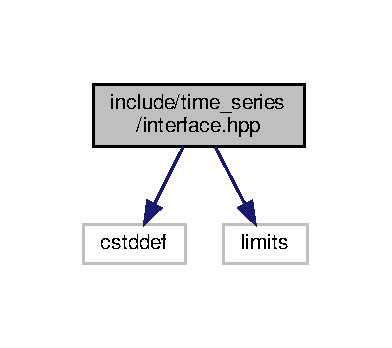
\includegraphics[width=188pt]{interface_8hpp__incl}
\end{center}
\end{figure}
This graph shows which files directly or indirectly include this file\+:
\nopagebreak
\begin{figure}[H]
\begin{center}
\leavevmode
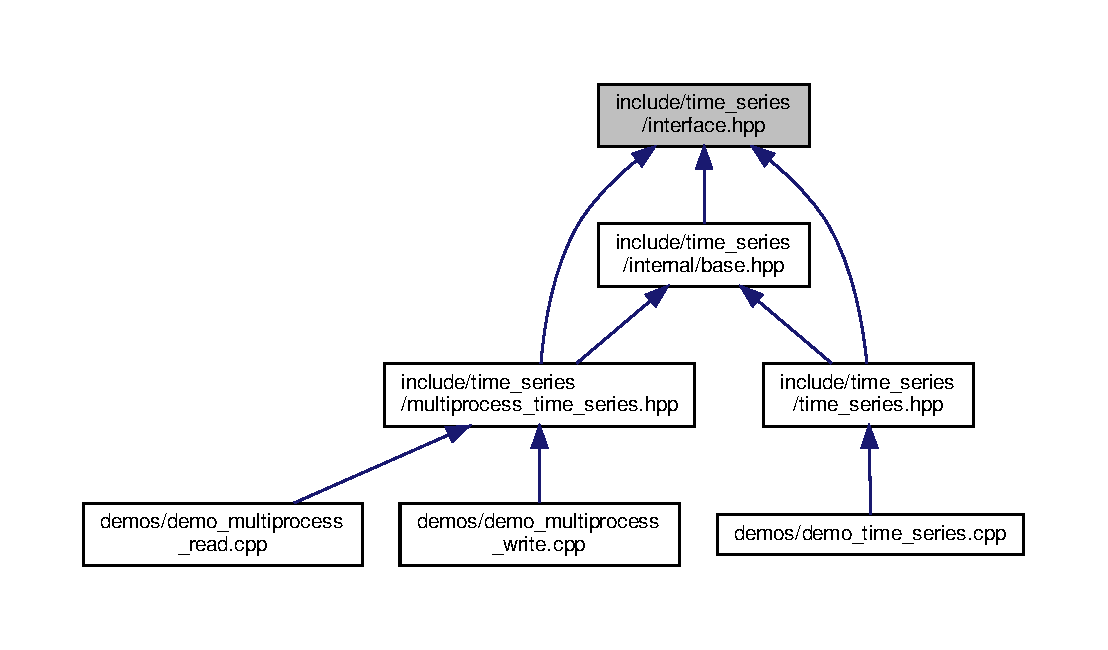
\includegraphics[width=350pt]{interface_8hpp__dep__incl}
\end{center}
\end{figure}
\subsection*{Classes}
\begin{DoxyCompactItemize}
\item 
class \hyperlink{classtime__series_1_1TimeSeriesInterface}{time\+\_\+series\+::\+Time\+Series\+Interface$<$ T $>$}
\begin{DoxyCompactList}\small\item\em Interface for time series. \end{DoxyCompactList}\end{DoxyCompactItemize}
\subsection*{Typedefs}
\begin{DoxyCompactItemize}
\item 
\mbox{\Hypertarget{interface_8hpp_a58076f07cd788dccb7a898fe711f8461}\label{interface_8hpp_a58076f07cd788dccb7a898fe711f8461}} 
typedef long int {\bfseries time\+\_\+series\+::\+Index}
\item 
\mbox{\Hypertarget{interface_8hpp_a5af99eebeeaa7402b16f6db135efe302}\label{interface_8hpp_a5af99eebeeaa7402b16f6db135efe302}} 
typedef long double {\bfseries time\+\_\+series\+::\+Timestamp}
\end{DoxyCompactItemize}
\subsection*{Variables}
\begin{DoxyCompactItemize}
\item 
\mbox{\Hypertarget{interface_8hpp_a56c6b210811506e9db80b703684ceee3}\label{interface_8hpp_a56c6b210811506e9db80b703684ceee3}} 
const Index {\bfseries time\+\_\+series\+::\+E\+M\+P\+TY} = -\/1
\end{DoxyCompactItemize}


\subsection{Detailed Description}
\begin{DoxyAuthor}{Author}
Vincent Berenz license License B\+S\+D-\/3-\/\+Clause 
\end{DoxyAuthor}
\begin{DoxyCopyright}{Copyright}
Copyright (c) 2019, Max Planck Gesellschaft. 
\end{DoxyCopyright}

\hypertarget{time__series_8hpp}{}\section{include/time\+\_\+series/time\+\_\+series.hpp File Reference}
\label{time__series_8hpp}\index{include/time\+\_\+series/time\+\_\+series.\+hpp@{include/time\+\_\+series/time\+\_\+series.\+hpp}}
{\ttfamily \#include $<$chrono$>$}\newline
{\ttfamily \#include $<$cmath$>$}\newline
{\ttfamily \#include \char`\"{}real\+\_\+time\+\_\+tools/timer.\+hpp\char`\"{}}\newline
{\ttfamily \#include \char`\"{}time\+\_\+series/interface.\+hpp\char`\"{}}\newline
{\ttfamily \#include \char`\"{}time\+\_\+series/internal/base.\+hpp\char`\"{}}\newline
{\ttfamily \#include \char`\"{}time\+\_\+series/internal/specialized\+\_\+classes.\+hpp\char`\"{}}\newline
Include dependency graph for time\+\_\+series.\+hpp\+:
\nopagebreak
\begin{figure}[H]
\begin{center}
\leavevmode
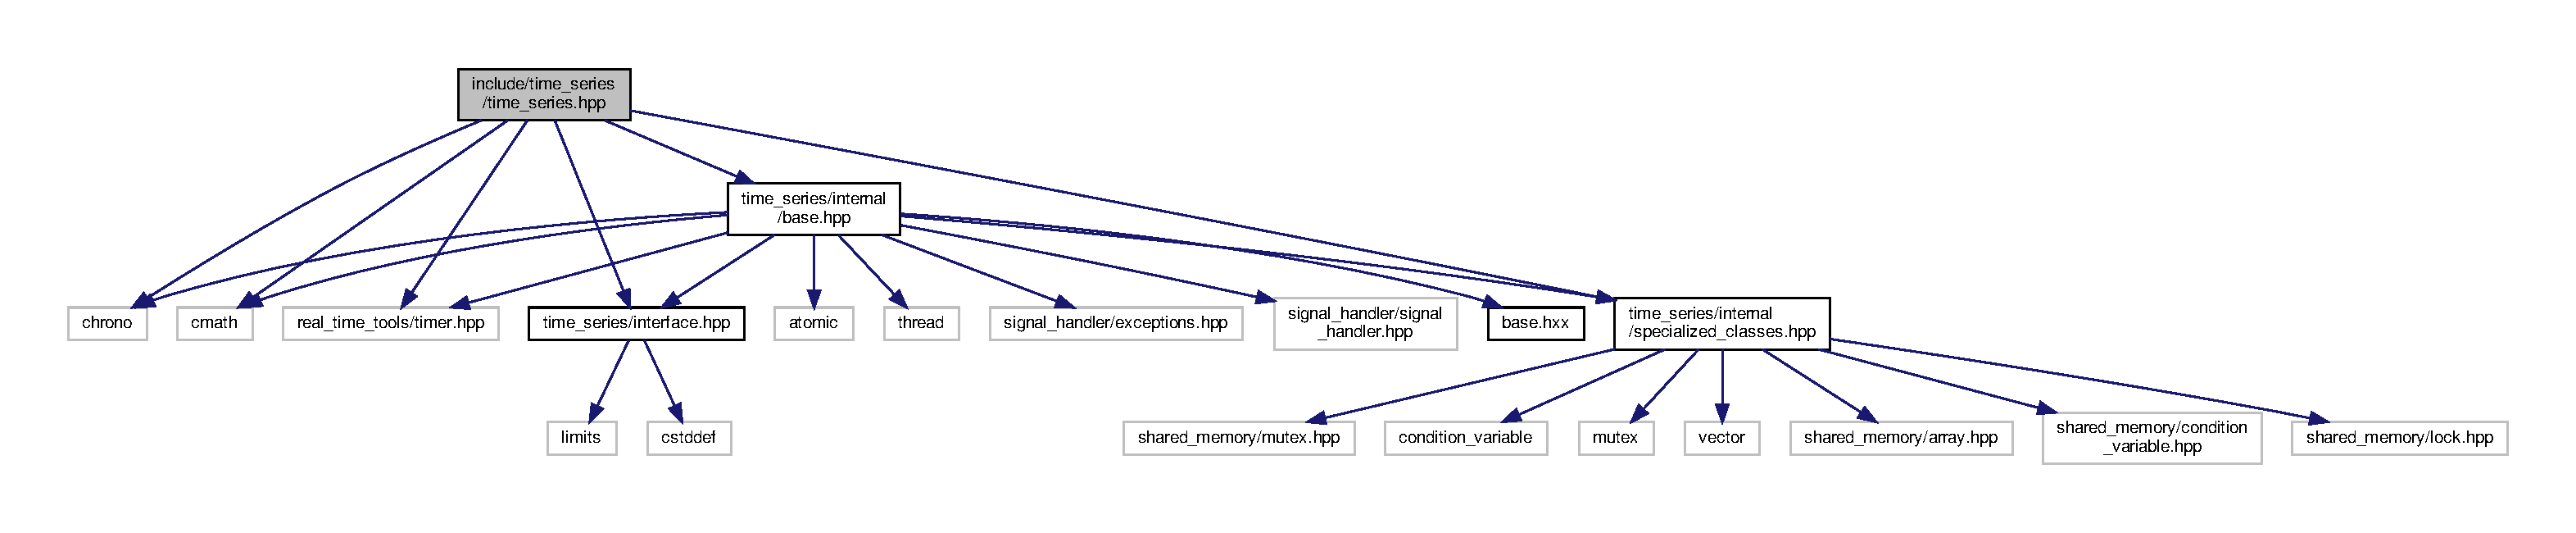
\includegraphics[width=350pt]{time__series_8hpp__incl}
\end{center}
\end{figure}
This graph shows which files directly or indirectly include this file\+:
\nopagebreak
\begin{figure}[H]
\begin{center}
\leavevmode
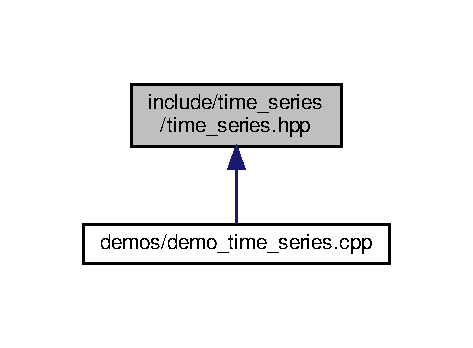
\includegraphics[width=227pt]{time__series_8hpp__dep__incl}
\end{center}
\end{figure}
\subsection*{Classes}
\begin{DoxyCompactItemize}
\item 
class \hyperlink{classtime__series_1_1TimeSeries}{time\+\_\+series\+::\+Time\+Series$<$ T $>$}
\begin{DoxyCompactList}\small\item\em Threadsafe time series. \end{DoxyCompactList}\end{DoxyCompactItemize}


\subsection{Detailed Description}
\begin{DoxyAuthor}{Author}
Vincent Berenz license License B\+S\+D-\/3-\/\+Clause 
\end{DoxyAuthor}
\begin{DoxyCopyright}{Copyright}
Copyright (c) 2019, Max Planck Gesellschaft. 
\end{DoxyCopyright}

%--- End generated contents ---

% Index
\backmatter
\newpage
\phantomsection
\clearemptydoublepage
\addcontentsline{toc}{chapter}{Index}
\printindex

\end{document}
